\documentclass[prd,twocolumn,nofootinbib,superscriptaddress,amsmath,amssymb]{revtex4-2}

\usepackage{graphicx}
\usepackage{bm}
\usepackage{booktabs}
\usepackage[colorlinks=true,allcolors=blue]{hyperref}

\newcommand{\dd}{\mathrm{d}}
\newcommand{\rhomf}{\rho_{\rm mf}}
\newcommand{\rhoopt}{\rho_{\rm opt}}
\newcommand{\dref}{d_0}
\newcommand{\vs}{v_\star}
\newcommand{\ds}{d_\star}
\newcommand{\vmin}{v_{\min}}
\newcommand{\vmax}{v_{\max}}
\newcommand{\dmin}{d_{\min}}
\newcommand{\dmax}{d_{\max}}
\newcommand{\Lam}{\Lambda}
\newcommand{\Ibar}{\bar{I}}
\newcommand{\E}{\mathbb{E}}
\newcommand{\Var}{\mathrm{Var}}

\begin{document}

\title{Table-free distance marginalization of the gravitational-wave likelihood}

\author{Colm Talbot}
\affiliation{Princeton University, Princeton, New Jersey 08544, USA}

\date{October 21, 2026}

\begin{abstract}
Gravitational-wave inference routinely marginalizes the likelihood analytically over luminosity distance, usually by interpolating a precomputed two-dimensional lookup table. We show that, written in terms of the matched-filter signal-to-noise ratio and the inverse distance at which the likelihood peaks, the distance-marginalized likelihood is exactly a Gaussian smoothing of the prior density in inverse distance, multiplied by a known exponential factor. This form makes the physics of each signal-strength regime explicit. At high signal-to-noise ratio a truncated-normal factorization plus a Laplace correction is accurate to $\lesssim 4\times10^{-5}$ in $\ln\mathcal{L}$ at the default thresholds. When the prior dominates, a cumulant expansion in prior moments is accurate to $\lesssim 2\times10^{-5}$, given a range criterion that we show is necessary. Between these limits, a six-panel Gauss--Legendre rule adapted to the location and width of the likelihood peak is accurate to $\lesssim 6\times10^{-5}$. With and without analytic phase marginalization, the combined method is accurate to $\sim 10^{-5}$ in $\ln\mathcal{L}$ over the full range of signal-to-noise ratios. It needs no precomputation, evaluates in about a microsecond, and is differentiable.
\end{abstract}

\maketitle

\section{Introduction}

In Bayesian parameter estimation for compact-binary coalescences~\cite{Veitch2015,Ashton2019,RomeroShaw2020,Biwer2019,Thrane2019}, several extrinsic parameters can be marginalized analytically or semi-analytically, which lowers the dimension of the space the sampler must explore. Luminosity distance $d_L$ is a natural candidate: the gravitational-wave strain scales as $1/d_L$, so the log-likelihood is a quadratic function of $1/d_L$ for fixed values of all other parameters. Distance marginalization was introduced for rapid localization~\cite{Singer2016a,Singer2016b} and is now standard in general-purpose inference codes~\cite{Thrane2019,Ashton2019,RomeroShaw2020}. It is also a building block of more aggressive marginalization schemes~\cite{Pankow2015,Lange2018,Roulet2024}.

The usual implementation tabulates the marginalized likelihood on a two-dimensional grid of the inner products $\langle d|h\rangle$ and $\langle h|h\rangle$, evaluated at a reference distance, and interpolates it during sampling~\cite{Thrane2019,Roulet2024}. A table is simple and fast, but it has four drawbacks. It must be rebuilt for every prior, which takes tens of seconds for the default grid in the \textsc{Bilby} library~\cite{Ashton2019}. Its interpolation error grows with signal strength, because the integrand sharpens as the signal-to-noise ratio (SNR) increases while the grid stays fixed. It covers only a finite domain. And it is not readily differentiable or portable across array libraries.

In this paper we derive a table-free alternative. The key step is a change of variables, Sec.~\ref{sec:likelihood}. In terms of the matched-filter SNR and the inverse distance at which the likelihood peaks, the marginalized likelihood factors exactly into a known exponential and a Gaussian smoothing of the prior density in inverse distance. This form has clean limits at high SNR (Sec.~\ref{sec:high}) and when the prior dominates (Sec.~\ref{sec:low}), and between them it is well suited to a small, peak-adapted quadrature (Sec.~\ref{sec:medium}). Section~\ref{sec:selection} gives the rule that selects among the three, Sec.~\ref{sec:validation} validates the accuracy and speed of the method, and Sec.~\ref{sec:implementation} summarizes two independent implementations.

\section{The distance-marginalized likelihood}
\label{sec:likelihood}

\subsection{Likelihood ratio as a function of distance}

For stationary Gaussian noise with one-sided power spectral density $S(f)$, the log-likelihood ratio of a signal $h$ against pure noise is~\cite{CutlerFlanagan1994,Thrane2019}
\begin{equation}
\ln\Lam \equiv \ln\frac{\mathcal{L}}{\mathcal{Z}_N} = \mathrm{Re}\langle d|h\rangle - \tfrac12\langle h|h\rangle,
\end{equation}
with the noise-weighted inner product
\begin{equation}
\langle a|b\rangle = 4\int_0^\infty \frac{\tilde a^*(f)\,\tilde b(f)}{S(f)}\,\dd f,
\end{equation}
where $\mathcal{Z}_N$ is the noise-only likelihood. All other parameters are held fixed, so the template depends on distance only through its amplitude, $h(d_L) = h_0\,\dref/d_L$, where $h_0$ is evaluated at an arbitrary reference distance $\dref$. Define
\begin{equation}
\rhoopt^2 \equiv \langle h_0|h_0\rangle,\qquad
\rhomf \equiv \frac{\mathrm{Re}\langle d|h_0\rangle}{\rhoopt},\qquad
v \equiv \frac{1}{d_L}.
\end{equation}
Here $\rhoopt$ is the optimal SNR at $\dref$, and $\rhomf$ is the matched-filter SNR, which is independent of both $d_L$ and $\dref$. The log-likelihood ratio is quadratic in $v$:
\begin{equation}
\ln\Lam(v) = A v - \tfrac12 B v^2,
\label{eq:lnlambda}
\end{equation}
with $A = \rhomf\rhoopt\dref$ and $B = (\rhoopt\dref)^2$.
Completing the square gives
\begin{equation}
\ln\Lam(v) = \frac{\rhomf^2}{2} - \frac{(v-\vs)^2}{2\sigma_v^2},
\label{eq:square}
\end{equation}
where
\begin{equation}
\vs = \frac{\rhomf}{\rhoopt\dref},\qquad \sigma_v = \frac{1}{\rhoopt\dref} = \frac{\vs}{\rhomf}.
\end{equation}
The maximum-likelihood distance is $\ds = 1/\vs$, and the likelihood is Gaussian in inverse distance with fractional width $1/\rhomf$. Its peak value, $\rhomf^2/2$, carries the dynamic range of the problem. The remaining factor varies only slowly, as we show below. If the template is anti-correlated with the data, then $\rhomf<0$ and $\vs<0$. Equation~\eqref{eq:square} still holds, but the peak then lies at negative inverse distance, outside any physical prior.

\subsection{Marginalization}

For a prior $\pi_d(d_L)$ on $[\dmin,\dmax]$, define the prior density in inverse distance, $\pi_v(v) = \pi_d(1/v)/v^2$, on $[\vmin,\vmax]=[1/\dmax,1/\dmin]$. Then
\begin{align}
\frac{\mathcal{L}_D}{\mathcal{Z}_N} &= \int \dd d_L\,\pi_d(d_L)\,\Lam(d_L) = e^{\rhomf^2/2}\,\mathcal{I},
\label{eq:identity}\\
\mathcal{I} &= \int_{\vmin}^{\vmax}\dd v\,\pi_v(v)\,e^{-(v-\vs)^2/2\sigma_v^2}.
\nonumber
\end{align}
This identity is exact. The quantity $\mathcal{I}$ is $\sqrt{2\pi}\sigma_v$ times the prior density in $v$ smoothed by a Gaussian of width $\sigma_v$ centred on $\vs$, so $0<\mathcal{I}\le1$. The large factor $e^{\rhomf^2/2}$ is analytic, and everything difficult about the problem lives in $\mathcal{I}$. To evaluate $\mathcal{I}$ without cancellation, we use the polynomial form of Eq.~\eqref{eq:lnlambda} directly. For example, when $\vs$ lies far outside the support, $\rhomf^2/2$ and the log of the Gaussian factor are large and nearly cancel.

\subsection{Phase marginalization}

For a dominant-mode signal, the complex overlap $z\equiv\langle d|h_0\rangle = |z|e^{i\psi}$ depends on the coalescence phase $\phi$ through $\mathrm{Re}\langle d|h_0\rangle = |z|\cos(2\phi-\psi)$, and $\langle h_0|h_0\rangle$ is independent of $\phi$. Averaging over a uniform phase prior gives $\int_0^{2\pi}\frac{\dd\phi}{2\pi}e^{|z| u\cos(2\phi-\psi)} = I_0(|z|u)$~\cite{Thrane2019}, where $u=\dref v$ and $I_0$ is the modified Bessel function. Redefining $\rhomf\equiv|z|/\rhoopt\ge0$, so that $A = |z|\dref$, and writing $I_0(x)=e^{x}\Ibar_0(x)$ in terms of the exponentially scaled $\Ibar_0$, the phase-marginalized integrand becomes
\begin{equation}
\pi_v(v)\,w(v)\,e^{-(v-\vs)^2/2\sigma_v^2},\qquad w(v)=\Ibar_0(Av).
\end{equation}
This has the form of Eq.~\eqref{eq:identity} with a slowly varying weight $w$. The weight satisfies $w\to1$ as $Av\to0$ and $w\simeq(2\pi Av)^{-1/2}$ for $Av\gg1$. Everything below covers both cases.

\subsection{Representation of the prior}

The method needs $\ln\pi_v$ and its first two derivatives anywhere on the support. Astrophysical distance priors are close to power laws, so we work in $s=\ln v$, where $g(s)\equiv\ln\pi_v(e^s)$ is nearly linear. We represent $g$ by a Chebyshev series on $[\ln\vmin,\ln\vmax]$~\cite{Trefethen2013}. The series is a least-squares fit to a dense tabulation of the prior, normalized so that $\int e^{g(s)+s}\dd s = 1$ (the factor $e^s$ is the Jacobian $\dd v=e^s\dd s$). Derivatives follow analytically from the Chebyshev derivative recurrence. For priors uniform in comoving volume and source-frame time, we tabulate the density directly from the cosmology:
\begin{equation}
\pi(z)\propto\frac{1}{1+z}\frac{\dd V_c}{\dd z},\qquad
\pi_d = \pi(z)\Big/\frac{\dd d_L}{\dd z},
\end{equation}
which avoids the kinks that an interpolated density would introduce. For the prior used throughout this paper, uniform in source frame on $[100,5000]$\,Mpc with Planck15 cosmology~\cite{Planck2016}, a degree-16 series fits $\ln\pi_v$ to a maximum residual of $5.5\times10^{-9}$. The prior moments $\E_\pi[v^k]$ needed in Sec.~\ref{sec:low} are computed once, by Gauss--Legendre quadrature.

\section{High signal-to-noise ratio}
\label{sec:high}

\subsection{Truncated-normal factorization}

Let $\alpha=(\vmin-\vs)/\sigma_v$ and $\beta=(\vmax-\vs)/\sigma_v$, and let $\bar v$ and $\Var_{\rm TN}$ be the mean and variance of the normal distribution $\mathcal{N}(\vs,\sigma_v)$ truncated to the support. With $f\equiv\pi_v w$, Eq.~\eqref{eq:identity} factors exactly as
\begin{equation}
\mathcal{I} = \underbrace{\sqrt{2\pi}\,\sigma_v[\Phi(\beta)-\Phi(\alpha)]}_{M}\;f(\bar v)\;R,
\qquad R = \frac{\E_{\rm TN}[f(v)]}{f(\bar v)},
\label{eq:factor}
\end{equation}
where $\Phi$ is the standard normal cumulative distribution. The Gaussian mass $M$ handles the peak itself, its passage through the prior edges, and the case in which the peak lies entirely outside the support. The remaining factor $R$ measures how far $f$ departs from linearity across the truncated normal, which is a Jensen-type correction.

\subsection{Laplace correction}

Write $f = e^{h}$ and $\delta = v-\bar v$. By construction $\E_{\rm TN}[\delta]=0$. Expanding $h$ about $\bar v$,
\begin{equation}
R = \E_{\rm TN}\!\left[e^{h'\delta + h''\delta^2/2 + \dots}\right]
= 1 + \tfrac12\Var_{\rm TN}\,(h''+h'^2) + \dots,
\end{equation}
so that
\begin{equation}
\ln R \simeq \tfrac12\,\Var_{\rm TN}\,\big[h''+h'^2\big]_{\bar v}.
\label{eq:laplace}
\end{equation}
The neglected terms involve the third and fourth central moments of the truncated normal and higher derivatives of $h$. In the interior of the support they are suppressed by further powers of the fractional width $\Var_{\rm TN}^{1/2}/\bar v$. In terms of $s$,
\begin{equation}
h' = \frac{g'}{v} + (\ln w)',\qquad h'' = \frac{g''-g'}{v^2} + (\ln w)'',
\end{equation}
with $(\ln w)' = A(r-1)$ and $(\ln w)'' = A^2(1 - r/x - r^2)$. Here $x=Av$, $r = I_1(x)/I_0(x)$, and $r/x\to\frac12$ as $x\to0$.

\paragraph{Interior limit.}
When the peak is well inside the support, $\bar v\to\vs$ and $\Var_{\rm TN}\to\sigma_v^2$. Since $\pi_v(\vs)\sigma_v = \pi_d(\ds)\,\ds/\rhomf$, without phase marginalization
\begin{equation}
\frac{\mathcal{L}_D}{\mathcal{Z}_N} \simeq e^{\rhomf^2/2}\,\sqrt{2\pi}\,\frac{\pi_d(\ds)\,\ds}{\rhomf}\,
\left[1 + \frac{\sigma_v^2}{2}\frac{\pi_v''(\vs)}{\pi_v(\vs)}\right].
\label{eq:interior}
\end{equation}
This is the familiar result of Laplace's method~\cite{BenderOrszag1978}: the peak likelihood multiplied by the ratio of the posterior width to the prior width, an Occam factor. For a power-law prior $\pi_d\propto d_L^{\,a}$, $\pi_v\propto v^{-(a+2)}$, and the correction is exactly $\ln R = (a+2)(a+3)/(2\rhomf^2)$. This equals $10/\rhomf^2$ for a prior uniform in Euclidean volume ($a=2$). With phase marginalization, $x\simeq\rhomf^2$ at the peak and $\Ibar_0(x)\simeq(2\pi x)^{-1/2}$, so the Occam factor becomes $\pi_d(\ds)\ds/\rhomf^2$.

\paragraph{Edge limit.}
If the peak lies beyond the support, for example $\vs>\vmax$ (the source is louder than allowed even at the closest distance $\dmin$), then $\beta\to-\infty$. The asymptotic form of the normal tail gives $M\simeq\lambda\,e^{-\beta^2/2}$, with
\begin{equation}
\lambda = \frac{\sigma_v^2}{|\vs-\vmax|},
\qquad
\frac{\mathcal{L}_D}{\mathcal{Z}_N} \simeq \Lam(\vmax)\,\pi_v(\vmax)\,\lambda.
\label{eq:edge}
\end{equation}
In words, the marginalized likelihood is the likelihood at the nearest allowed distance multiplied by the prior mass within one exponential decay length $\lambda$ of the edge. The same expression with $\vmin$ applies to $\rhomf<0$. The template is then anti-correlated with the data, the likelihood increases monotonically towards infinite distance, and the integral is dominated by the far edge of the prior.

\subsection{Stable truncated-normal moments}

The textbook expressions for $\bar v$ and $\Var_{\rm TN}$~\cite{JohnsonKotz1994} cancel catastrophically in the tails. For example, when $\alpha\gg1$ the variance is $\simeq\sigma_v^2/\alpha^2$, but it is computed as a difference of terms of order $\sigma_v^2\alpha^2$. We orient the interval so that its endpoint nearer to $\vs$ is the standardized lower limit $a\ge0$, and write $t = x - a$. The truncated density is then proportional to $e^{-at-t^2/2}$. Its moments follow from three functions, $m(a)$, $u(a)$ and $w(a)$, which are the zeroth to second moments of that kernel on $[0,\infty)$. They are computed without cancellation from Laplace's continued fraction~\cite{AbramowitzStegun1964}, as detailed in Appendix~\ref{app:tn}. The resulting moments are accurate to within a few units of machine precision for any $\alpha,\beta$. The naive formula, by contrast, gives a variance with an order-unity relative error already at $\alpha\sim10^4$.

\subsection{Range of validity}

The expansion~\eqref{eq:laplace} is used when $|\rhomf|\ge30$ and the fractional width satisfies $\Var_{\rm TN}^{1/2}\le0.01\,\bar v$. Across four priors and both phase settings, these thresholds bound its error by $4\times10^{-5}$. The second condition matters only far outside the support, where the truncated distribution can be broad even at large $\rhomf$.

\section{Prior-dominated limit}
\label{sec:low}

\subsection{Cumulant expansion}

When the likelihood varies little across the prior support, it is natural to expand about the prior itself. Writing $X\equiv\ln\Lam(v)$,
\begin{equation}
\frac{\mathcal{L}_D}{\mathcal{Z}_N} = \E_\pi\!\left[e^{X}\right],
\qquad
\ln\frac{\mathcal{L}_D}{\mathcal{Z}_N} = \sum_{n\ge1}\frac{\kappa_n}{n!},
\label{eq:cumulant}
\end{equation}
where $\kappa_n$ are the cumulants of $X$ under the prior, so that Eq.~\eqref{eq:cumulant} is the cumulant generating function evaluated at unit argument. To first order, $\ln\mathcal{L}_D/\mathcal{Z}_N\simeq A\langle v\rangle - B\langle v^2\rangle/2$, the prior-averaged log-likelihood ratio. The second order adds half its prior variance. Because $X$ is a polynomial in $v$, every raw moment of $X$ is a polynomial in $(A,B)$ whose coefficients are prior moments $\E_\pi[v^k]$. These are computed once, so the series needs no table. In practice we expand about the prior mean, in the scaled variable $v/\vmax$, using central moments of the prior. This avoids cancellation between the large raw moments of $X$.

\subsection{Phase marginalization}

With phase marginalization, $X = \ln I_0(Av) - Bv^2/2$ is no longer polynomial in $v$. The power series of $\ln I_0$ follows from the logarithm of $I_0(x)=\sum_k (x^2/4)^k/(k!)^2$:
\begin{multline}
\ln I_0(x) = \frac{x^2}{4}-\frac{x^4}{64}+\frac{x^6}{576}-\frac{11x^8}{49152}\\
+\frac{19x^{10}}{614400}-\frac{473x^{12}}{106168320}+\dots
\end{multline}
This makes $X$ a polynomial in $v^2$, and the expansion~\eqref{eq:cumulant} goes through unchanged with prior moments of $v^2$. The series converges for $|x|<j_{0,1}\simeq2.405$, the modulus of the zeros of $I_0$ on the imaginary axis. We keep six terms and require $A\vmax\le1$, where the truncation error is below $10^{-6}$.

\subsection{When the expansion fails}

The cumulant series is asymptotic rather than convergent, and the obvious control variable, $\kappa_2=\Var_\pi[X]$, is not sufficient on its own. A prior that places most of its mass at large distances can coexist with a sharp likelihood peak at small distances. That peak can dominate $\E_\pi[e^X]$ while contributing almost nothing to the low-order cumulants. For example, take a source-frame prior on $[10,5\times10^4]$\,Mpc, with $\rhomf = 21.5$ and $\ds = 2.7$\,Mpc. Then $\kappa_2 = 0.033$, yet $X$ spans 107\,nats across the support, and the truncated series is wrong by 85\,nats. We therefore require both $\kappa_2<0.05$ and that the range of $X$ over the support be at most one nat. With these conditions and the series truncated at fourth order, the error is below $2\times10^{-5}$ in all our tests.

\section{Intermediate signal-to-noise ratio}
\label{sec:medium}

\subsection{Physical picture}

Between the two limits, neither expansion applies. The Gaussian in Eq.~\eqref{eq:identity} is too broad for the Laplace correction to be small: at $\rhomf\sim$ a few, $\ln R$ is of order one to ten for steep priors. Yet it is far too narrow for the likelihood to be treated as a perturbation of the prior. This regime contains a qualitatively distinct feature. As $d_L\to\infty$ the template vanishes and $\Lam\to1$, while at the peak $\Lam = e^{\rhomf^2/2}$. Astrophysical priors place most of their mass at large distances, so the far tail of the prior can contribute a fraction of order $e^{-\rhomf^2/2}\,P_\pi(\text{far})$ of the integral. For $\rhomf\lesssim$ a few this produces a second mode in the conditional distance posterior. A Laplace expansion about the peak misses that mode, and a cumulant expansion cannot resolve the peak. The integral must be computed with a quadrature that resolves both features.

\subsection{Peak-adapted quadrature}

We integrate in $s=\ln v$, where the prior is smooth. The integrand is
\begin{equation}
F(s) = \exp\!\left[g(s) + s + A e^s - \tfrac12 B e^{2s} + \ln w(e^s)\right].
\end{equation}
Its sharpest feature is the Gaussian peak, so we place breakpoints relative to the peak location $c=\mathrm{clip}(\vs,\vmin,\vmax)$ and a scale
\begin{equation}
\ell = \frac{\sigma_v^2}{\max(\sigma_v,\Delta)},\qquad \Delta = |\vs-c|.
\end{equation}
Inside the support, $\ell=\sigma_v$, the Gaussian width. Outside it, $\ell=\lambda$, the exponential decay length of Eq.~\eqref{eq:edge}. The breakpoints are $c+\{-40,-8,0,8,40\}\ell$, clipped to the support and mapped to $s$. Together with the two support edges they define six panels, each integrated with a 20-point Gauss--Legendre rule~\cite{GolubWelsch1969}, for 120 integrand evaluations in total:
\begin{itemize}
\item The inner panels, of width $\pm8\ell$, contain the peak, where the integrand is a Gaussian (or exponential) times a smooth function.
\item The next panels follow the tail down to $e^{-40}$ of its peak value.
\item The outer panels extend to the edges of the support and contain only the smooth prior multiplied by a slowly varying likelihood. This captures the far-distance mode described above.
\end{itemize}
All of these integrands are analytic, so Gauss--Legendre quadrature converges geometrically in the number of nodes. On our calibration sets, the worst error over the whole intermediate regime is $1.0\times10^{-3}$, $5.8\times10^{-5}$, $2.6\times10^{-6}$ and $3.2\times10^{-9}$ for 16, 20, 24 and 32 nodes per panel. We use 20 nodes.

Two details make the rule cheap and differentiable. First, $\ln\pi_v$ is needed at every node. We evaluate it by cubic Hermite interpolation on 64 uniformly spaced knots in $s$, using the exact Chebyshev values and first derivatives at the knots. The interpolation error is $O(h^4)$ and adds less than $10^{-6}$. Second, each panel is reduced with a log-sum-exp, and the panels are combined linearly with their half-widths as weights. A panel that collapses to zero width, which happens when a breakpoint is clipped to an edge, then keeps the correct derivative with respect to its breakpoints. This preserves gradients when $\vs$ lies exactly on a prior edge.

\section{Regime selection and continuity}
\label{sec:selection}

\begin{table*}
\caption{\label{tab:thresholds}Default regime-selection thresholds and the worst error of each branch over the calibration sets: four priors, both phase settings, $\ds\in[\dmin/5,5\dmax]$, $|\rhomf|\in[10^{-3},10^4]$.}
\begin{ruledtabular}
\begin{tabular}{lll}
Branch & Condition & Worst $|\Delta\ln\mathcal{L}|$\\
\hline
Cumulant (4th order) & $\kappa_2<0.05$, range$(X)\le1$ & $2\times10^{-5}$\\
 & (phase: also $A\vmax\le1$) & \\
High SNR & $|\rhomf|\ge30$, $\Var_{\rm TN}^{1/2}\le0.01\,\bar v$ & $4\times10^{-5}$\\
Quadrature & otherwise (6 panels $\times$ 20 nodes) & $6\times10^{-5}$\\
\end{tabular}
\end{ruledtabular}
\end{table*}

The three branches are selected in a fixed order. The cumulant expansion is used if its conditions hold. Otherwise the high-SNR expansion is used if its conditions hold, and otherwise the quadrature. Table~\ref{tab:thresholds} summarizes the conditions. Figure~\ref{fig:regimes} shows the resulting partition of the $(\ds,\rhomf)$ plane for the source-frame prior on $[100,5000]$\,Mpc:
\begin{itemize}
\item the high-SNR expansion covers $\rhomf\gtrsim30$;
\item the cumulant expansion covers the region where the likelihood is nearly flat across the prior, at $\rhomf\lesssim1$ for sources inside the support, extending to larger $\rhomf$ when $\ds\gg\dmax$;
\item the quadrature covers the band between them.
\end{itemize}
Every branch has an error far below the target, so the jump in $\ln\mathcal{L}$ across any regime boundary is below $10^{-4}$. We verified this by scanning lines that cross every boundary.

\begin{figure*}
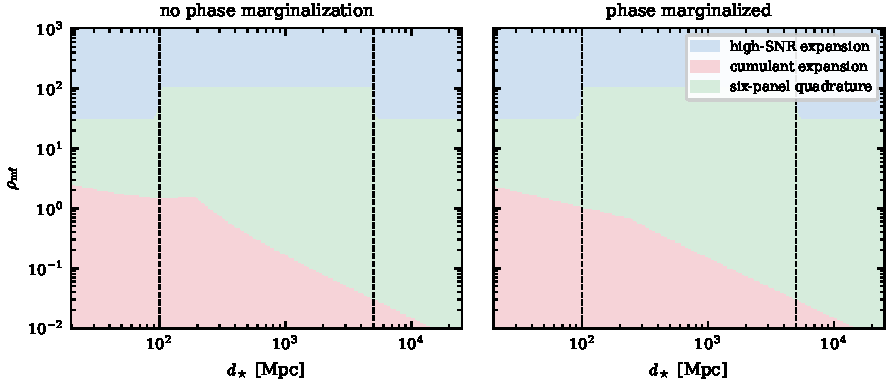
\includegraphics[width=\textwidth]{figures/regime_map.pdf}
\caption{\label{fig:regimes}Evaluation regime across the plane of maximum-likelihood distance $\ds$ and matched-filter SNR $\rhomf$, for the source-frame prior on $[100,5000]$\,Mpc (dashed lines). Left: without phase marginalization. Right: with phase marginalization.}
\end{figure*}

\section{Validation}
\label{sec:validation}

\subsection{Accuracy}

Figure~\ref{fig:limiting} follows a single line through the plane, with $\ds = 1000$\,Mpc and $\rhomf$ from $10^{-2}$ to $10^3$. It shows the two limiting forms converging onto the exact result in their respective regimes, and the quadrature accurate throughout. The error of the selected branch along this line is at most $2\times10^{-7}$ without phase marginalization and $3\times10^{-7}$ with it. The errors of the two expansions grow quickly outside their regimes, reaching order one below $\rhomf\sim1$ for the high-SNR expansion and above $\rhomf\sim3$ for the cumulant expansion. This is why both conditions in Table~\ref{tab:thresholds} are needed.

\begin{figure*}
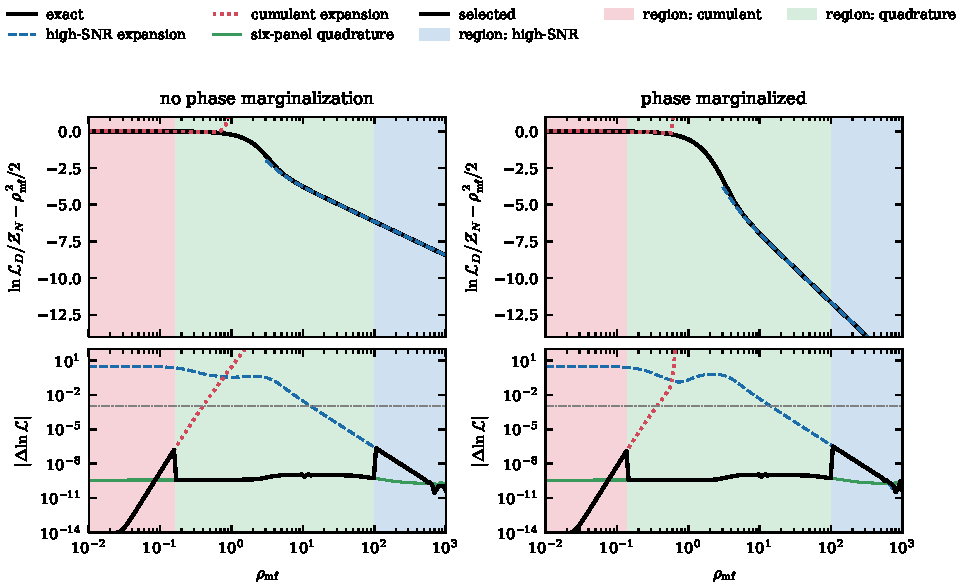
\includegraphics[width=\textwidth]{figures/limiting_forms.pdf}
\caption{\label{fig:limiting}Limiting forms of the distance-marginalized likelihood for $\ds=1000$\,Mpc. Top: $\ln(\mathcal{L}_D/\mathcal{Z}_N)-\rhomf^2/2=\ln\mathcal{I}$ (black), compared with the high-SNR expansion, Eqs.~\eqref{eq:factor}--\eqref{eq:laplace}, and the cumulant expansion, Eq.~\eqref{eq:cumulant}. Bottom: absolute error of each branch, evaluated everywhere regardless of the selection rule, and of the selected branch (thick black). Shading marks the selected regime. The dash-dotted line marks $10^{-3}$.}
\end{figure*}

Figure~\ref{fig:accuracy} summarizes the error over a grid of 924 points, with $\rhomf\in[0.1,10^3]$ and $\ds\in[20,2.5\times10^4]$\,Mpc. These include sources far outside the prior support. Without (with) phase marginalization, the worst error is $1.2\times10^{-5}$ ($1.6\times10^{-5}$) and the median is $5\times10^{-10}$. For comparison, the \textsc{Bilby} lookup table for the same prior has a median error of $7.7\times10^{-4}$ ($6.7\times10^{-4}$). Inside the prior support its error is at most $1.6\times10^{-3}$ for $\rhomf<10$, grows to $\sim0.2$ for $\rhomf\sim10$--$100$, and exceeds several nats above $\rhomf\sim100$, where the integrand is much sharper than the table grid. Outside its tabulated domain the interpolant returns $-\infty$, which happens for 24 of the 924 points. In both comparisons the reference is a dense composite Gauss--Legendre quadrature of the same continuous prior.

\begin{figure*}
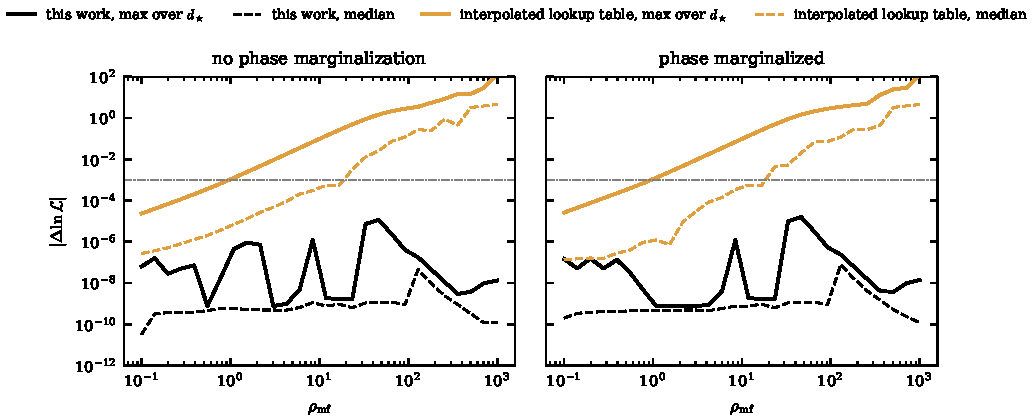
\includegraphics[width=\textwidth]{figures/accuracy.pdf}
\caption{\label{fig:accuracy}Accuracy as a function of SNR: worst-case (solid) and median (dashed) error over $\ds\in[20,2.5\times10^4]$\,Mpc, for this method (black) and an interpolated lookup table (orange, \textsc{Bilby}'s default $400\times800$ table), for the source-frame prior on $[100,5000]$\,Mpc. Points at which the table returns $-\infty$ are omitted from its curves.}
\end{figure*}

As an independent check, we compared against arbitrary-precision quadrature (25 significant digits, \textsc{mpmath}~\cite{mpmath}) of the analytic priors themselves rather than of their tabulations. We used 104 query points per prior, chosen to cover the interior, the edges, the exterior and negative $\rhomf$, for four priors: source-frame on $[100,5000]$ and $[10,5\times10^4]$\,Mpc, and $\pi_d\propto d_L^2$ and $\pi_d\propto d_L^{-1}$ on $[50,5000]$\,Mpc. The worst error over all priors and both phase settings is $1.2\times10^{-5}$.

\subsection{End-to-end inference}

We repeated a standard injection study with \textsc{Bilby}:
\begin{itemize}
\item a binary black hole injected at $d_L = 2000$\,Mpc into two-detector Advanced LIGO noise, recovered with a log Bayes factor of $\approx75$ against noise;
\item IMRPhenomPv2 waveforms;
\item a source-frame distance prior on $[100,5000]$\,Mpc;
\item the chirp mass, mass ratio and inclination sampled, with distance marginalized;
\item the \textsc{dynesty} nested sampler with 500 live points.
\end{itemize}
The run used an earlier quadrature setting of 32 nodes per panel, whose likelihood differs from the default by less than $10^{-4}$.

Over 100 draws from the prior and 100 draws near the injection, the marginalized likelihood agreed with a brute-force distance integral to $1.2\times10^{-6}$. The lookup table differed from it by up to $10^{-2}$. Table~\ref{tab:inference} compares the evidence and the reconstructed distance posterior. The two methods agree to within sampling noise, with a Kolmogorov--Smirnov $p$-value of 0.12 for the distance samples.

\begin{table}
\caption{\label{tab:inference}End-to-end comparison in an injection study (injected $d_L=2000$\,Mpc).}
\begin{ruledtabular}
\begin{tabular}{lcc}
 & This method & Lookup table\\
\hline
$\ln\mathcal{Z}$ & $-8026.56\pm0.16$ & $-8026.94\pm0.16$\\
$d_L$ median [Mpc] & 1773 & 1718\\
$d_L$ 90\% interval [Mpc] & [1196, 2542] & [1181, 2541]\\
Injected-value quantile & 0.64 & 0.65\\
\end{tabular}
\end{ruledtabular}
\end{table}

\subsection{Cost}

Figure~\ref{fig:timing} shows the cost per evaluation across SNR on an Apple M2 Ultra CPU. The cost follows the selected regime:
\begin{itemize}
\item In the compiled implementation, a single scalar evaluation takes 0.6\,$\mu$s in the high-SNR regime and about 1.8\,$\mu$s in the quadrature regime. It is cheaper at low SNR, falling to 0.8\,$\mu$s at $\rhomf=0.1$, where most sources use the cumulant expansion.
\item A single interpolation of the lookup table takes about 8\,$\mu$s. In a sampler, which evaluates the likelihood one point at a time, the method is therefore four to thirteen times faster than the table.
\item For batches of $10^4$ points, the compiled implementation takes 70--240\,ns per point, against 240--390\,ns per point for the table.
\item The array-API implementation compiled with JAX runs at about 380\,ns per point on CPU, and supports automatic differentiation.
\end{itemize}
The method needs no precomputation beyond a fit of the prior, which takes a few milliseconds. The default lookup table takes about 40\,s to build for each phase setting.

\begin{figure}
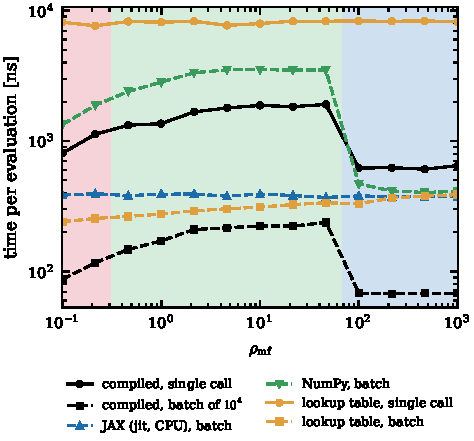
\includegraphics[width=\columnwidth]{figures/timing.pdf}
\caption{\label{fig:timing}Cost per evaluation versus SNR for sources uniformly distributed in $\ln\ds$ within the prior support, without phase marginalization. Background shading marks the majority regime (colors as in Fig.~\ref{fig:regimes}).}
\end{figure}

\section{Implementation}
\label{sec:implementation}

We provide two implementations of the method, written independently from a common specification:
\begin{itemize}
\item a Python package that evaluates in the array namespace of its inputs (NumPy, JAX~\cite{Jax2018}, PyTorch~\cite{Paszke2019}), following the Python array API standard~\cite{ArrayAPI}, and supports just-in-time compilation, vectorization and automatic differentiation;
\item a Rust library, also exposed to Python as a compiled backend for NumPy inputs.
\end{itemize}
The two share no code. They use different least-squares solvers, quadrature-node algorithms and special-function implementations, and are compared only through data files. Their prior fits agree to $10^{-12}$, and their likelihoods agree to $\lesssim10^{-9}$ relative over $5\times10^4$ test queries, with identical regime selection. Both are freely available under the MIT license.

Two practical extensions follow directly from the formalism:
\begin{itemize}
\item \textbf{Distance reconstruction.} The conditional distance posterior is $p(d_L|\vec\theta,d)\propto\pi_d(d_L)\Lam(d_L)$, which can be sampled exactly by inverse-transform sampling on a grid concentrated around $\bar v$.
\item \textbf{Time marginalization.} Each time bin has its own $(\rhomf,\vs)$. The method is evaluated on an array over bins, and the results are combined with a log-sum-exp.
\end{itemize}

\section{Conclusions}

Writing the likelihood in terms of the matched-filter SNR and the peak inverse distance turns distance marginalization into the Gaussian smoothing of a one-dimensional prior density. Its exact factorization separates out the analytic dynamic range. The high-SNR and prior-dominated limits have transparent physical interpretations: an Occam factor, the likelihood at the prior edge multiplied by a decay length, and the prior-averaged likelihood. The intermediate regime, where the distance posterior can be bimodal, is handled by a small quadrature adapted to the peak. Together these give a table-free, differentiable evaluation, accurate to $\sim10^{-5}$ in $\ln\mathcal{L}$ at all SNRs, at a cost comparable to or below that of interpolating a precomputed table.

\begin{acknowledgments}
The software and this manuscript were developed with the assistance of an AI coding assistant (Claude, Anthropic). All results were checked against independent arbitrary-precision calculations.
\end{acknowledgments}

\appendix

\section{Truncated-normal moments without cancellation}
\label{app:tn}

Standardize the truncation limits to $[\alpha,\beta]$, and reflect $(\alpha,\beta)\to(-\beta,-\alpha)$ if $\alpha+\beta<0$, giving an interval $[a,b]$ with $a+b\ge0$.

If $a<0<b$, the interval contains the peak. The mass $Z=\Phi(b)-\Phi(a)$ is computed as $\ln Z=\ln\Phi(b)+\ln[1-e^{\ln\Phi(a)-\ln\Phi(b)}]$, evaluating $\ln(1-e^{y})$ stably~\cite{Maechler2012}. The standard expressions
\begin{align}
\E[x]&=r_a-r_b, & \Var[x]&=1+a r_a-b r_b-(r_a-r_b)^2,
\end{align}
with $r_{a,b}=\phi(a,b)/Z$, are then well conditioned.

If $a\ge0$, the interval lies in a tail. Shift to $t=x-a\in[0,L]$, with $L=b-a$, so that the density is proportional to $e^{-at-t^2/2}$. Define
\begin{equation}
\{m,u,w\}(a)=\int_0^\infty \{1,t,t^2\}\,e^{-at-t^2/2}\,\dd t .
\end{equation}
Here $m(a)$ is the Mills ratio, and integration by parts gives $u=1-am$ and $w=m-au$. For $a\ge3$ these differences cancel, so we use Laplace's continued fraction~\cite{AbramowitzStegun1964}:
\begin{equation}
m=\frac{1}{a+D_1},\qquad D_k=\frac{k}{a+D_{k+1}},
\end{equation}
which gives $u=mD_1$ and $w=mD_1D_2$ with no subtraction. Sixty levels reach machine precision for $a\ge3$, and $m$ is evaluated directly for $a<3$. With $q=e^{-aL-L^2/2}$, the moments on $[0,L]$ are
\begin{align}
I_0&=m_a-q\,m_b,\nonumber\\
I_1&=u_a-q\,(u_b+L\,m_b),\nonumber\\
I_2&=w_a-q\,(w_b+2L\,u_b+L^2m_b),
\end{align}
giving $\E[x]=a+I_1/I_0$, $\Var[x]=I_2/I_0-(I_1/I_0)^2$ and $\ln(\sqrt{2\pi}Z)=-a^2/2+\ln I_0$. For a one-sided tail ($q\to0$), the variance $w/m-(u/m)^2\simeq1/a^2$ is now a difference of terms of comparable size, so no precision is lost.

\section{Usage examples}
\label{app:api}

In Python, given a tabulated prior and the inner products at a reference distance:
\begin{verbatim}
import numpy as np
from distmarg import DistanceMarginalization

d = np.geomspace(100, 5000, 4096)
dm = DistanceMarginalization(
    d, 2 * np.log(d),
    phase_marginalization=True)
rho_opt = np.sqrt(h_inner_h)
ln_l = dm.ln_likelihood_ratio(
    d_inner_h / rho_opt,
    rho_opt, d_ref)
\end{verbatim}
Here \texttt{d\_inner\_h} and \texttt{h\_inner\_h} are $\langle d|h\rangle$ and $\langle h|h\rangle$ at the reference distance. The inputs may be NumPy, JAX or PyTorch arrays of any broadcastable shape, and the result is returned in the same array namespace. In Rust:
\begin{verbatim}
use distmarg::{
    Config, DistanceMarginalization};

let dm = DistanceMarginalization::new(
    &d, &ln_prior, true,
    Config::default())?;
let ln_l = dm.ln_likelihood_ratio(
    rho_mf, rho_opt, d_ref);
\end{verbatim}

\bibliography{references}

\end{document}
